
\begin{frame}{Evoluci\'on de los instrumentos en cabina}
  
  \begin{tabular}{ccc}
    {\bf \large 1903} & & {\bf \large 1916} \\ & & \\
	{Wright Flyer I} & & {Fokker D.VII} \\ & & \\
    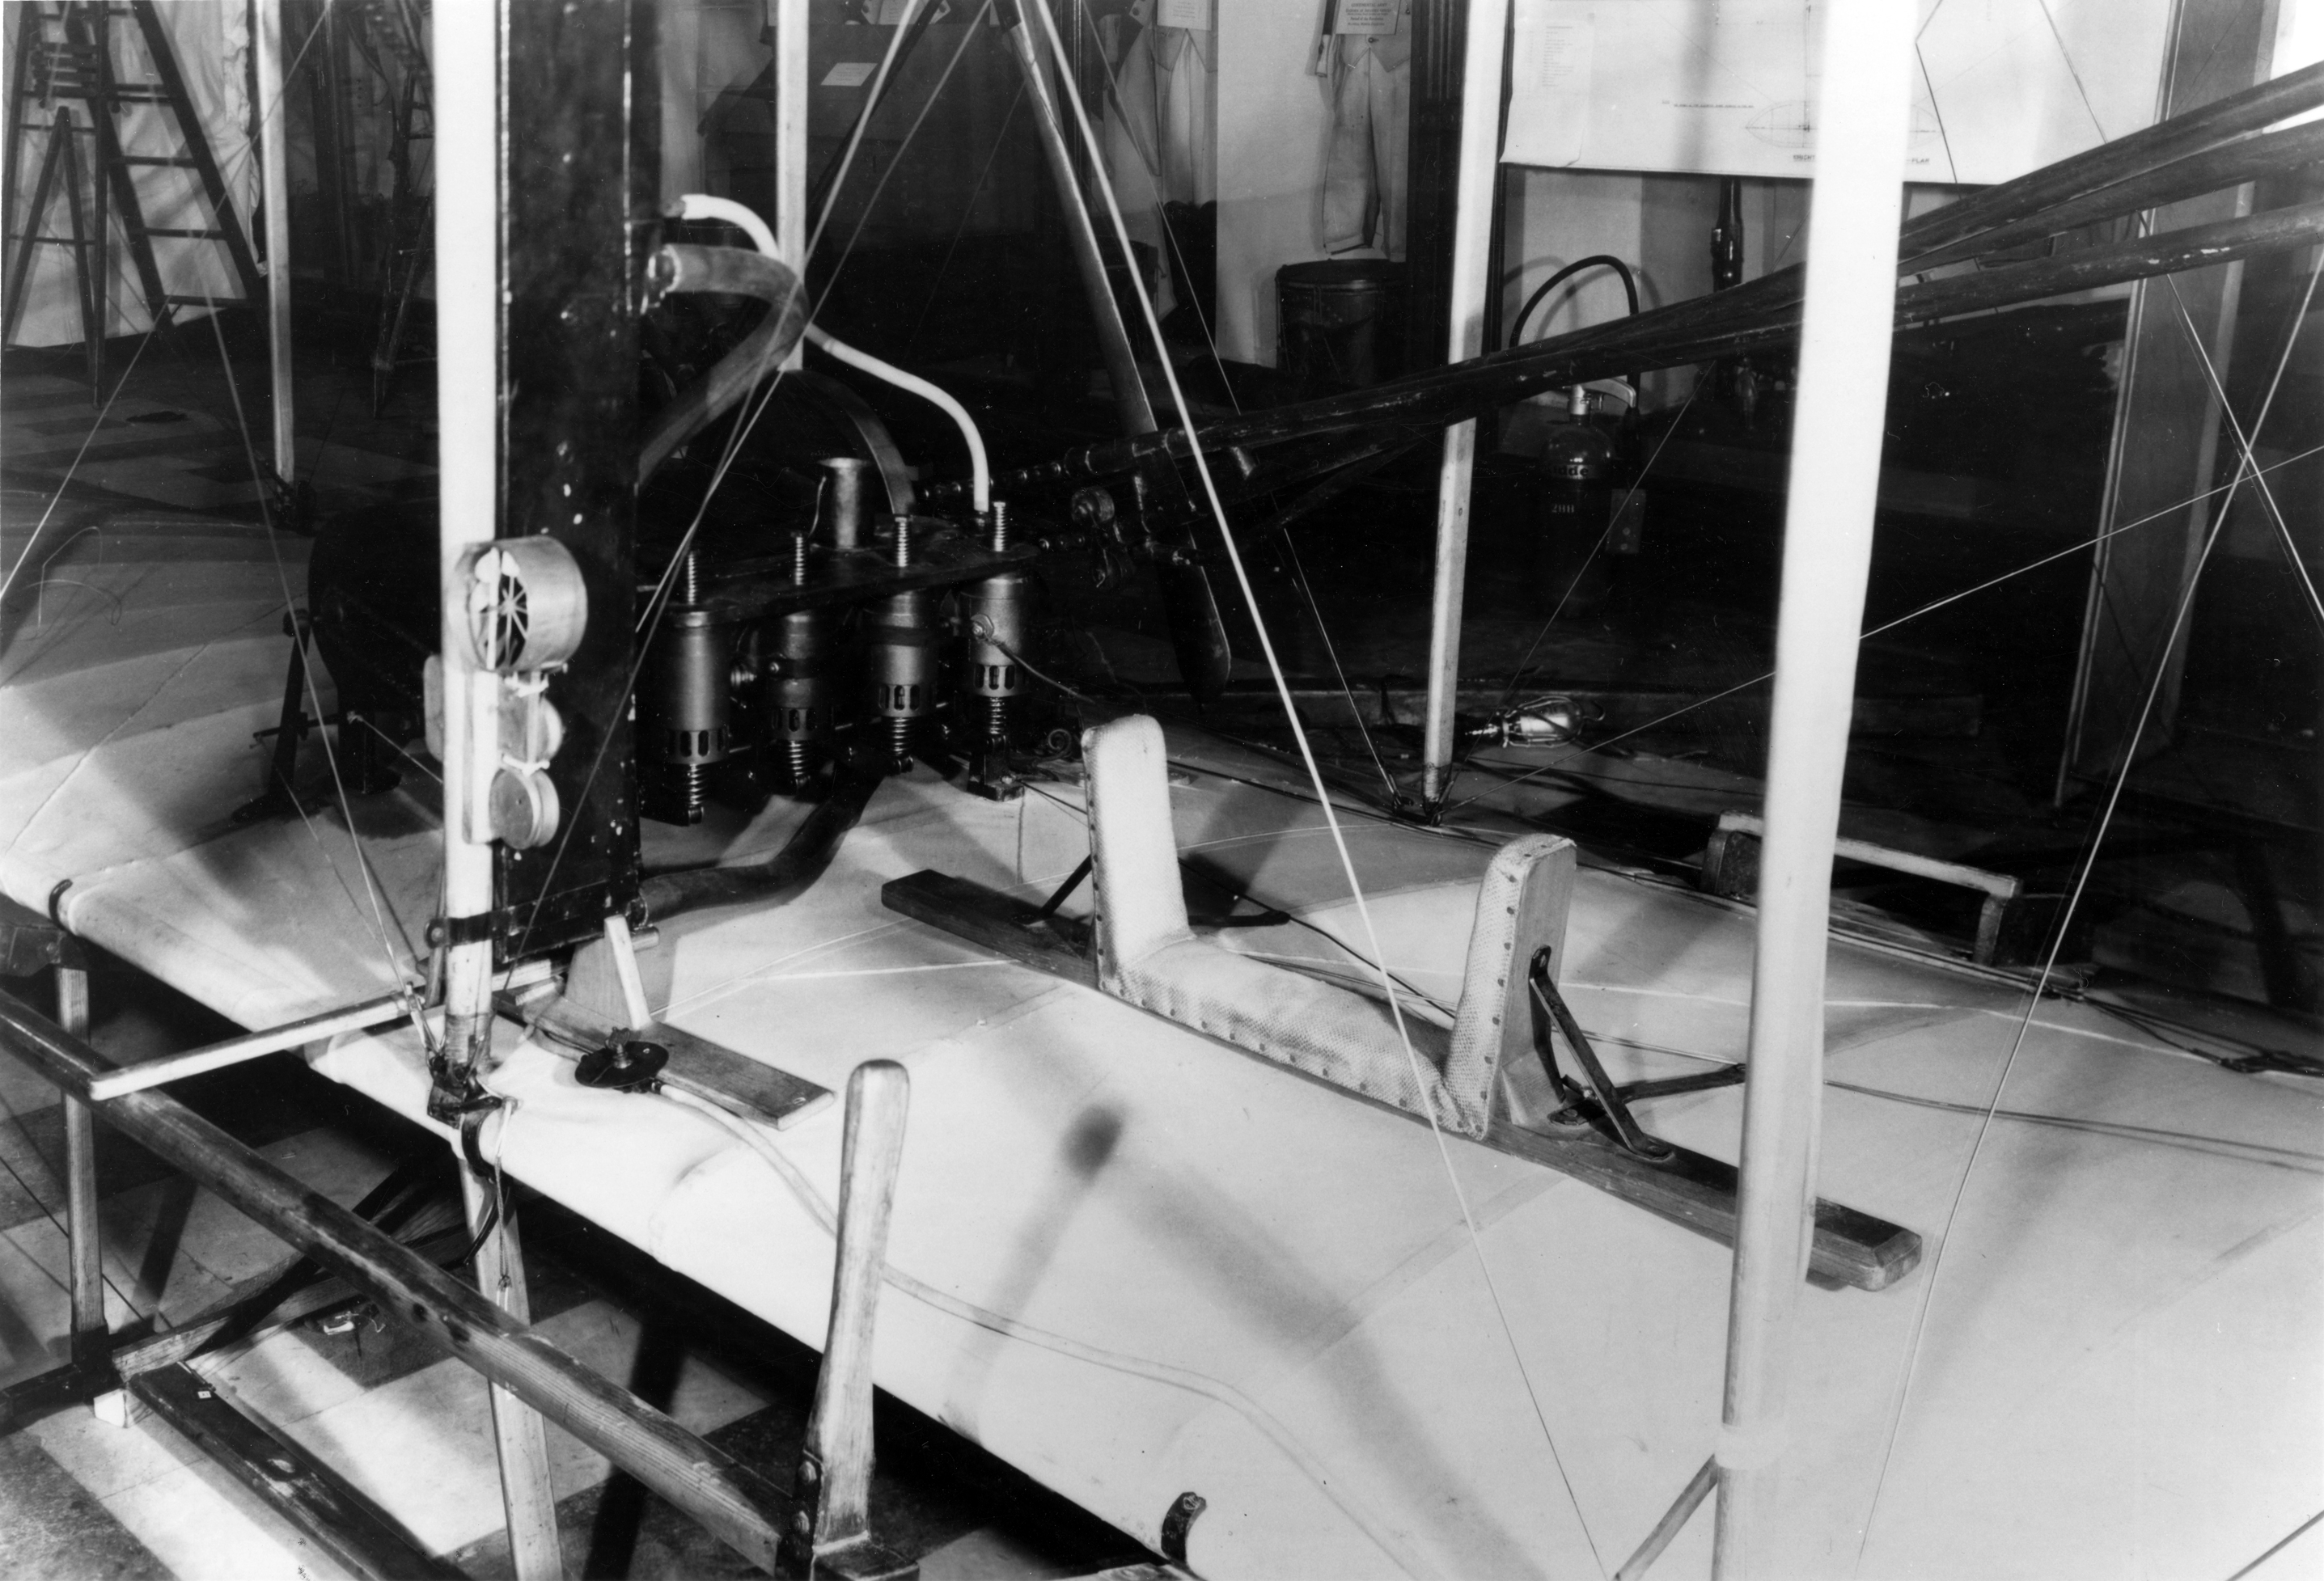
\includegraphics[width=0.45\textwidth]{imagenes/1.1.introduccion/wright_brothers_instruments.jpg}
	& \hspace{2.5mm}
	&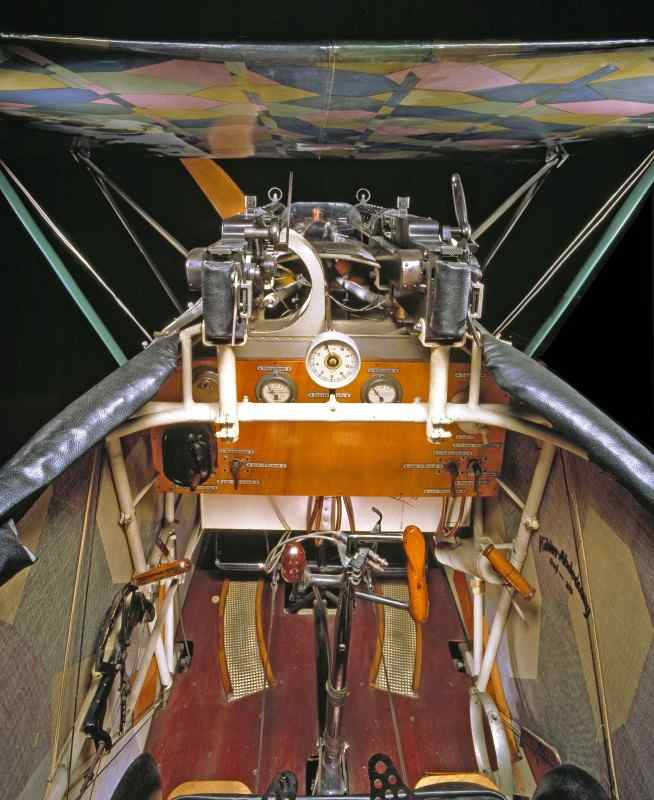
\includegraphics[width=0.35\textwidth]{imagenes/1.1.introduccion/005-fokker-d-vii.jpg} \\ & & \\
\parbox{0.4\textwidth}{\footnotesize
	Tres (3) instrumentos: \\
	\mbox{cron\'ometro}, anem\'ometro,\\ tac\'ometro}
	& & \\
	\multicolumn{3}{c}{
	{\tiny Fuente: \url{https://firstaerosquadron.com/2015/09/23/cockpit-evolution-from-the-beginning-to-present/}}}  \\
  \end{tabular}

\end{frame}


\begin{frame}{Evoluci\'on de los instrumentos en cabina}
  
  \begin{tabular}{ccc}
    {\bf \large 1916-1917} & & {\bf \large 1927} \\ & & \\
	{Jenny JN-4} & & {Spirit of St. Louis } \\ & & \\
    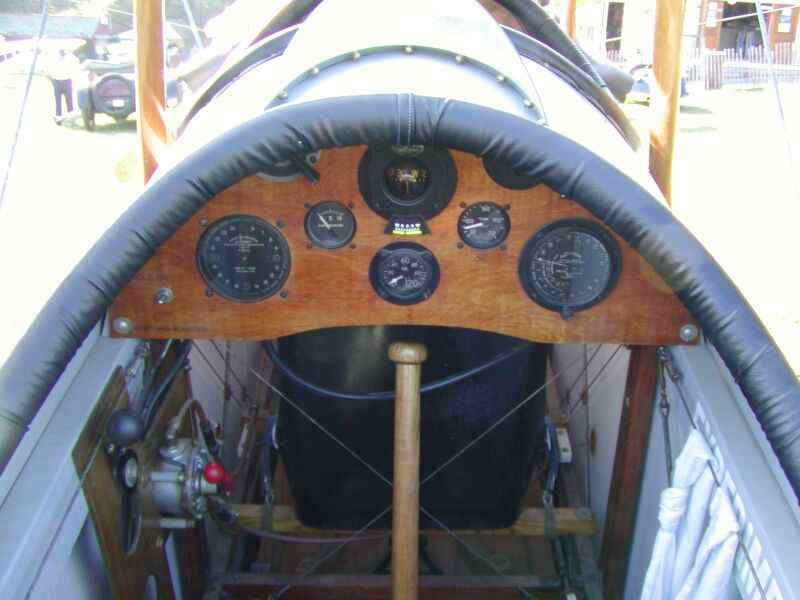
\includegraphics[width=0.35\textwidth]{imagenes/1.1.introduccion/curtiss_jenny_tablero.jpg}
	& \hspace{5mm}
	&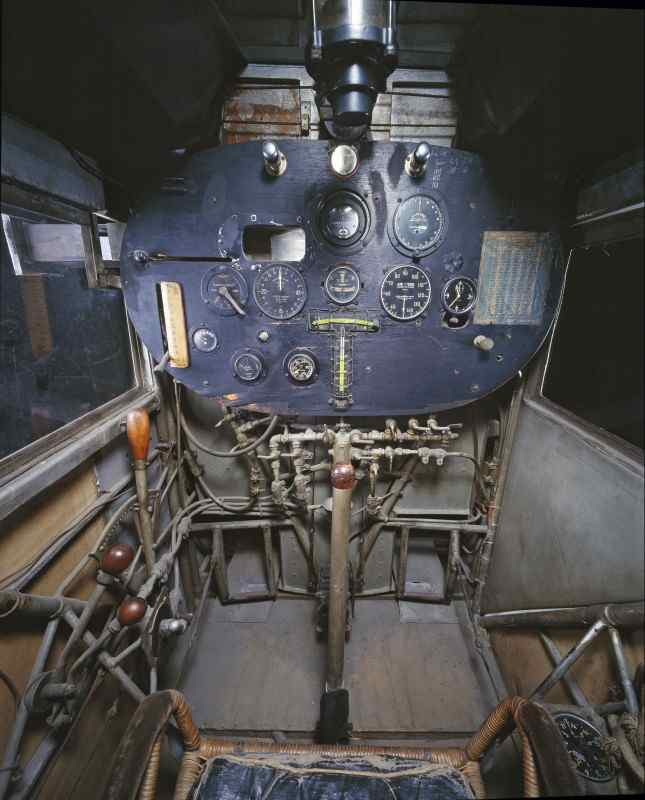
\includegraphics[width=0.35\textwidth]{imagenes/1.1.introduccion/002-lingbergs-spirit-of-st-louis.jpg} \\ & & \\
	\multicolumn{3}{l}{
	{\tiny Fuente: \url{https://firstaerosquadron.com/2015/09/23/cockpit-evolution-from-the-beginning-to-present/}}
}
	\\
  \end{tabular}

\end{frame}


\begin{frame}{Evoluci\'on de los instrumentos en cabina}
  
  \begin{tabular}{ccc}
    {\bf \large 1939} & & {\bf \large 1945} \\ & & \\
	{Supermarine Spitffire Mk VII} & & {Messerschmitt Me-262 } \\ & & \\
    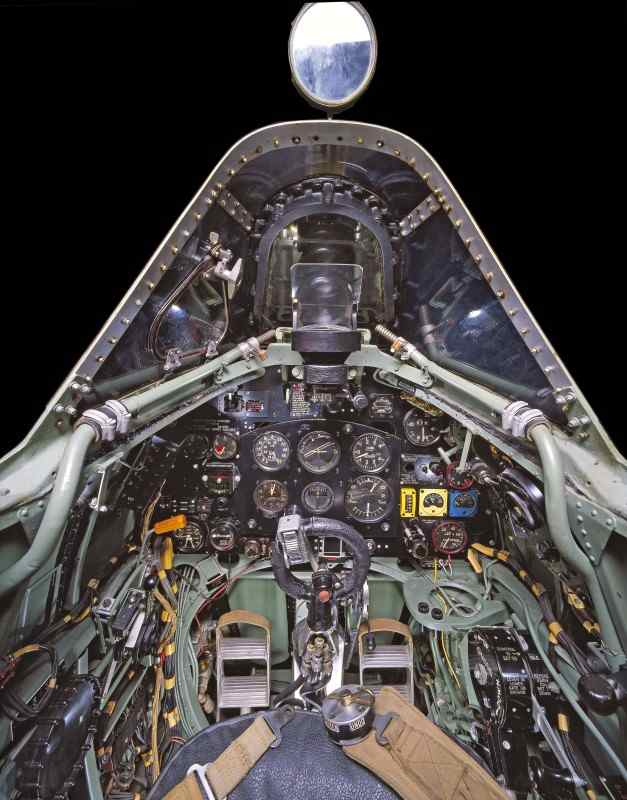
\includegraphics[width=0.35\textwidth]{imagenes/1.1.introduccion/006-supermarine-spitfire-mk-vii.jpg}
	& \hspace{5mm}
	&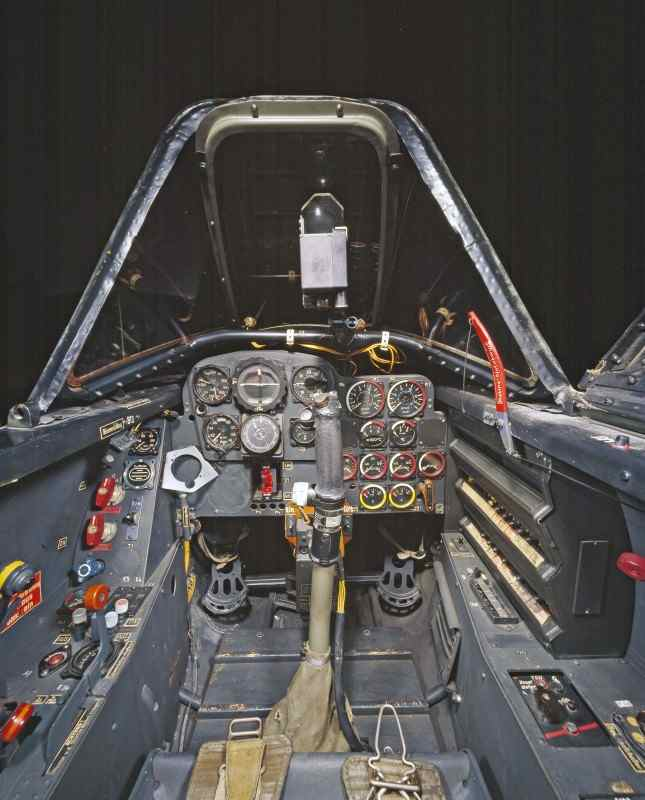
\includegraphics[width=0.35\textwidth]{imagenes/1.1.introduccion/008-messerschmitt-me-262a-1a.jpg} \\ & & \\
	\multicolumn{3}{l}{
	{\tiny Fuente: \url{https://firstaerosquadron.com/2015/09/23/cockpit-evolution-from-the-beginning-to-present/}}
}
	\\
  \end{tabular}

\end{frame}


\begin{frame}{Evoluci\'on de los instrumentos en cabina}
  
  \begin{tabular}{ccc}
    {\bf \large 1949} & & {\bf \large 1953} \\ & & \\
	{De Havilland Comet } & & {Douglas DC-7} \\ & & \\
    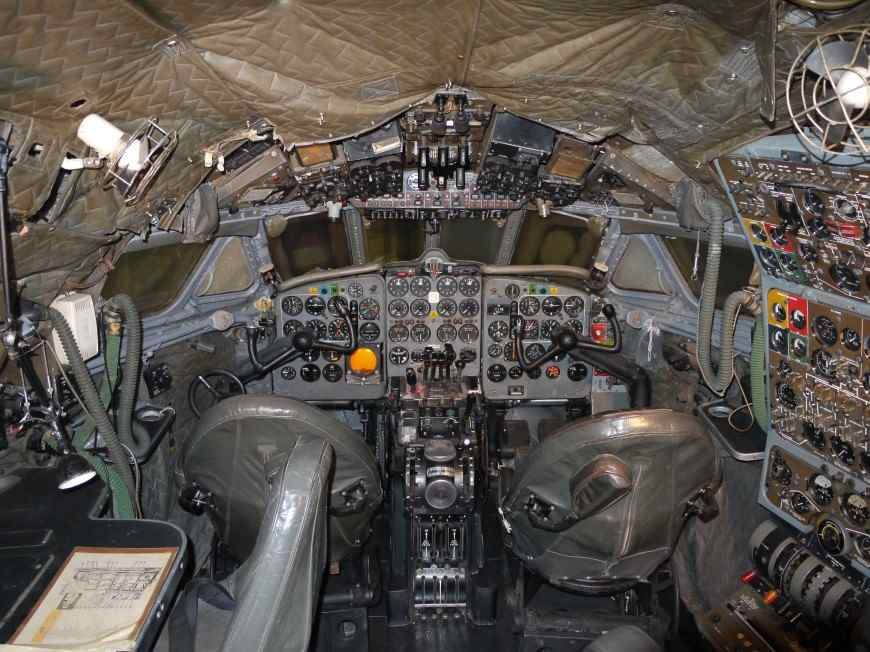
\includegraphics[width=0.35\textwidth]{imagenes/1.1.introduccion/012-de-havilland-dh-106-comet-1st-commercial-jet-airliner.jpg}
	& \hspace{5mm}
	&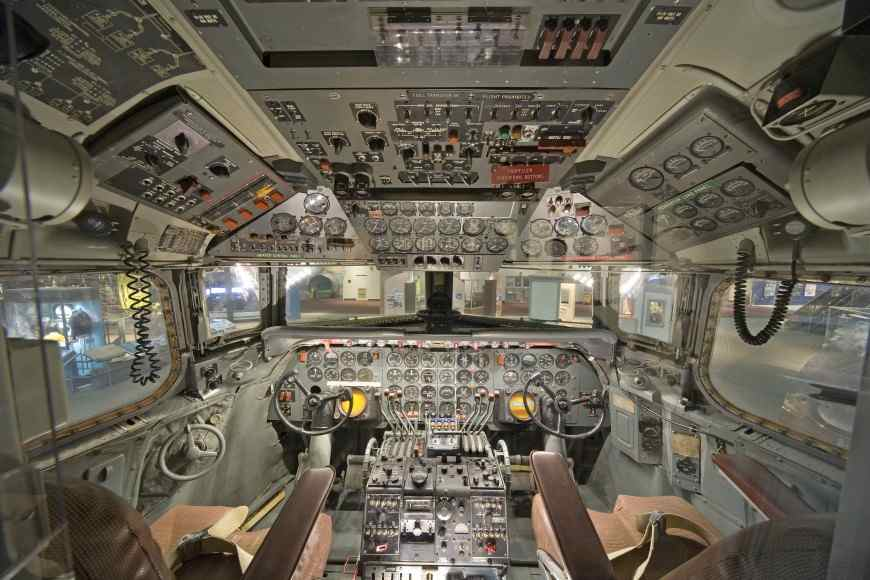
\includegraphics[width=0.35\textwidth]{imagenes/1.1.introduccion/015-douglas-dc-7.jpg} \\ & & \\
	\multicolumn{3}{l}{
	{\tiny Fuente: \url{https://firstaerosquadron.com/2015/09/23/cockpit-evolution-from-the-beginning-to-present/}}
}
	\\
  \end{tabular}

\end{frame}


\begin{frame}{Evoluci\'on de los instrumentos en cabina}
  
  \begin{tabular}{ccc}
    {\bf \large 1968} & & {\bf \large 1969} \\ & & \\
	{Lockheed SR-71 } & & {Concorde} \\ & & \\
    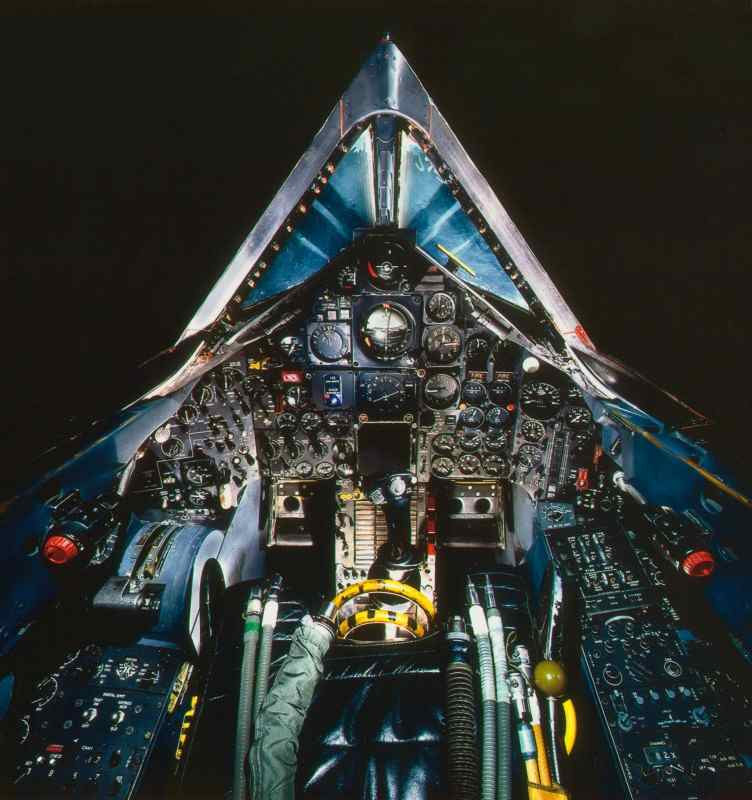
\includegraphics[width=0.35\textwidth]{imagenes/1.1.introduccion/014-lockheed-sr-71a-fas-blackbird.jpg}
	& \hspace{5mm}
	&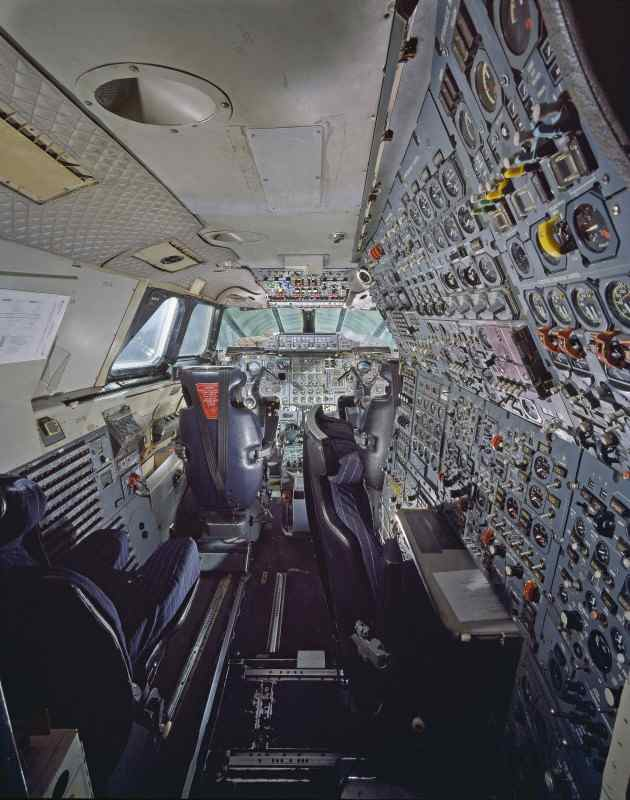
\includegraphics[width=0.35\textwidth]{imagenes/1.1.introduccion/017-concorde.jpg} \\ & & \\
	\multicolumn{3}{l}{
	{\tiny Fuente: \url{https://firstaerosquadron.com/2015/09/23/cockpit-evolution-from-the-beginning-to-present/}}
}
	\\
  \end{tabular}

\end{frame}




\begin{frame}{Evoluci\'on de los instrumentos en cabina}
  
  \begin{tabular}{ccc}
    {\bf \large 2005} & & {\bf \large 2009} \\ & & \\
	{Airbus A380} & & {Boeing 787 ``Dreamliner'' } \\ & & \\
    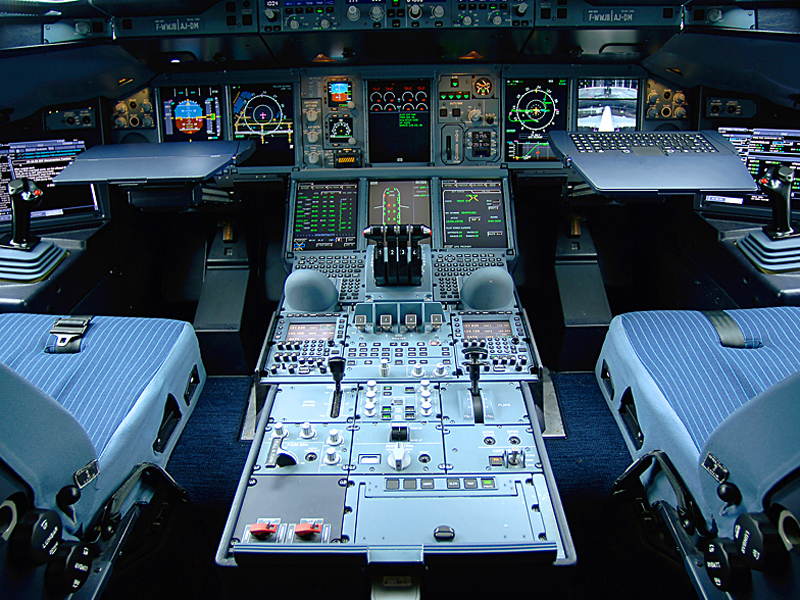
\includegraphics[width=0.45\textwidth]{imagenes/1.1.introduccion/A380_Cockpit_2.jpg}
	& \hspace{5mm}
	&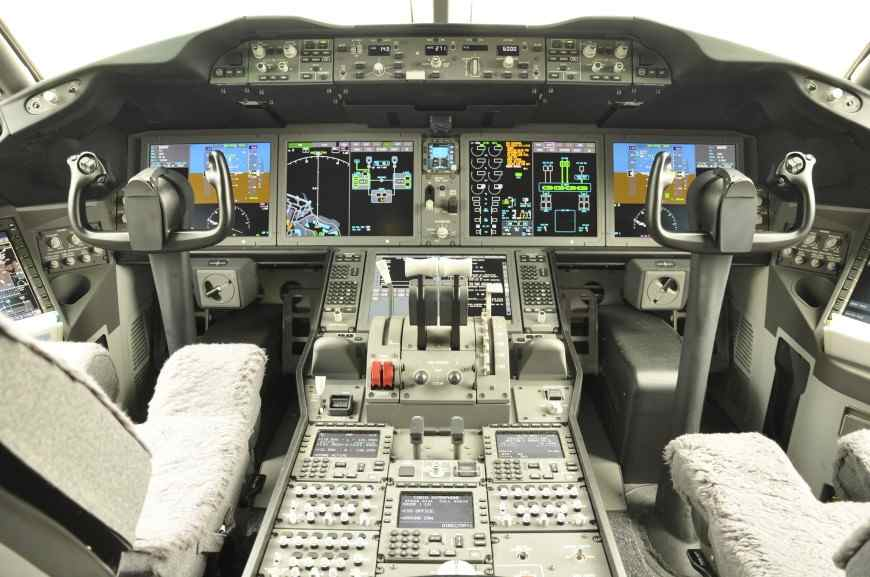
\includegraphics[width=0.45\textwidth]{imagenes/1.1.introduccion/019-boeing-787.jpg} \\ & & \\
	\multicolumn{3}{l}{
	{\tiny Fuente: \url{https://firstaerosquadron.com/2015/09/23/cockpit-evolution-from-the-beginning-to-present/}}
}
	\\
  \end{tabular}

\end{frame}
